% updated April 2002 by Antje Endemann
% Based on CVPR 07 and LNCS, with modifications by DAF, AZ and elle, 2008 and AA, 2010, and CC, 2011; TT, 2014; AAS, 2016; AAS, 2020

% \documentclass[runningheads]{llncs}
% \documentclass[arXiv_main.tex]{subfiles}
\documentclass[crop=false]{standalone}

\usepackage{graphicx}
\usepackage{hyperref}
% DO NOT USE \usepackage{times}, it will be removed by typesetters
%\usepackage{times}

\usepackage{tikz}
\usepackage{comment} 
\usepackage{amsmath,amssymb} % define this before the line numbering.
\usepackage{color}

\usepackage{graphicx}
\usepackage{multirow}
\usepackage{bm}
\usepackage{float}

\definecolor{yang_olive}{rgb}{0.5,0.5,0} 
\definecolor{del_gray}{rgb}{0.8,0.8,0.8} 
\newcommand\pjl[1]{\textcolor{black}{#1}}
\newcommand\peng[1]{\textcolor{black}{#1}}
\newcommand\wca[1]{\textcolor{black}{#1}}
\newcommand\wfb[1]{\textcolor{black}{#1}}
\newcommand\deleted[1]{\textcolor{del_gray}{#1}}
\newcommand\old[1]{\textcolor{orange}{\textit{#1}}}
\newcommand{\yang}[1]{\textcolor{black}{#1}}
\newcommand{\rev}[1]{\textcolor{blue}{#1}}

% \newcommand\CRpjl[1]{\textcolor{red}{#1}}
% \newcommand\CRpeng[1]{\textcolor{black}{#1}}
% \newcommand\CRwca[1]{\textcolor{pink}{#1}}
% \newcommand\CRwfb[1]{\textcolor{blue}{#1}}
% \newcommand{\CRyang}[1]{\textcolor{yang_olive}{#1}}

\newcommand\CRpjl[1]{\textcolor{black}{#1}}
\newcommand\CRpeng[1]{\textcolor{black}{#1}}
\newcommand\CRwca[1]{\textcolor{black}{#1}}
\newcommand\CRwfb[1]{\textcolor{black}{#1}}
\newcommand{\CRyang}[1]{\textcolor{black}{#1}}


% INITIAL SUBMISSION - The following two lines are NOT commented
% CAMERA READY - Comment OUT the following two lines
%\usepackage{ruler}
%\usepackage[width=122mm,left=12mm,paperwidth=146mm,height=193mm,top=12mm,paperheight=217mm]{geometry}


% \renewcommand\footnotemark{}
% \renewcommand\footnoterule{}
\usepackage{lipsum}
\newcommand\blfootnote[1]{%
\begingroup
\renewcommand\thefootnote{}\footnote{#1}%
\addtocounter{footnote}{-1}%
\endgroup
}


\begin{document}
% \renewcommand\thelinenumber{\color[rgb]{0.2,0.5,0.8}\normalfont\sffamily\scriptsize\arabic{linenumber}\color[rgb]{0,0,0}}
% \renewcommand\makeLineNumber {\hss\thelinenumber\ \hspace{6mm} \rlap{\hskip\textwidth\ \hspace{6.5mm}\thelinenumber}}
% \linenumbers
\pagestyle{headings}
\mainmatter
\def\ECCVSubNumber{100}  % Insert your submission number here

\title{Polyhedral Active Recognition
} % 

% INITIAL SUBMISSION 
\begin{comment}
\titlerunning{ECCV-20 submission ID \ECCVSubNumber} 
\authorrunning{ECCV-20 submission ID \ECCVSubNumber} 
\author{Anonymous ECCV submission}
\institute{Paper ID \ECCVSubNumber}
\end{comment}
%******************

% CAMERA READY SUBMISSION
%\begin{comment}
% \titlerunning{Chained-Tracker}
% If the paper title is too long for the running head, you can set
% an abbreviated paper title here
%
\author{Sajjad Pakdamansavoji (savoji@yorku.ca)
}

%
% \authorrunning{Sajjad Pakdamansav}
% First names are abbreviated in the running head.
% If there are more than two authors, 'et al.' is used.
%
% \institute{York University \quad
% \email{savoji@yorku.ca}
% }
%\end{comment}
%******************
\maketitle



\begin{abstract}
This report is written for the final project of Advanced Computer Vision course at York University. The aim of this challenge is to implement an active vision solution for distinguishing amongst sinle polyhedrals.
\\ 

In short My solution consists of four main modules: observation, feature extraction, comparison, active motion policy. Observation module receives a camera position and object ID from the Active Policy module and presents an image of the object. Feature extraction takes in the observation and creates informative features from it. Comparison module takes in those features and decides whether the two objects are the same. Such decision is then propagated to the Active Motion Policy where the next observation position is created. The result of my implementation is submitted for evaluation; it follows an original idea and presents a reasonable structure. My code is publicly available at \url{https://github.com/SajjadPSavoji/Active-Polyhedral-Scene-Matching}.

\end{abstract}


\section{Introduction}
Existing computer vision challenges(such as image net\cite{deng2009imagenet}) heavily emphasize on static object recognition; however when the 3D point-could of objects are projected into the image plane a large proportion of information is thrown away causing ambiguity for recovering the 3D structure. Some works suggest using additional sensory input such as LIDAR to compensate at least a proportion of that missing information. Although such approaches are useful and practical, recognizing objects should better be addressed in an active fashion since the physical constraints of an object imposes the necessity of obtaining multiple view-points to recover the 3D-structure and hence recognize the target fully. 
\\

\noindent In this study we wish to showcase the imortance of active vision; as such, the task in hand is using simple polyhedral objects. These objects are synthesized using Random Polyhedral Scenes \cite{2018arXiv180310100S} which was developed at York University. This scene generator creates a random object based on a few user parameters, renders the scene from random view points and creates a dataset containing the renderings and corresponding annotation files \ref{fig:RPS}.

\begin{figure*}[t]
\centering
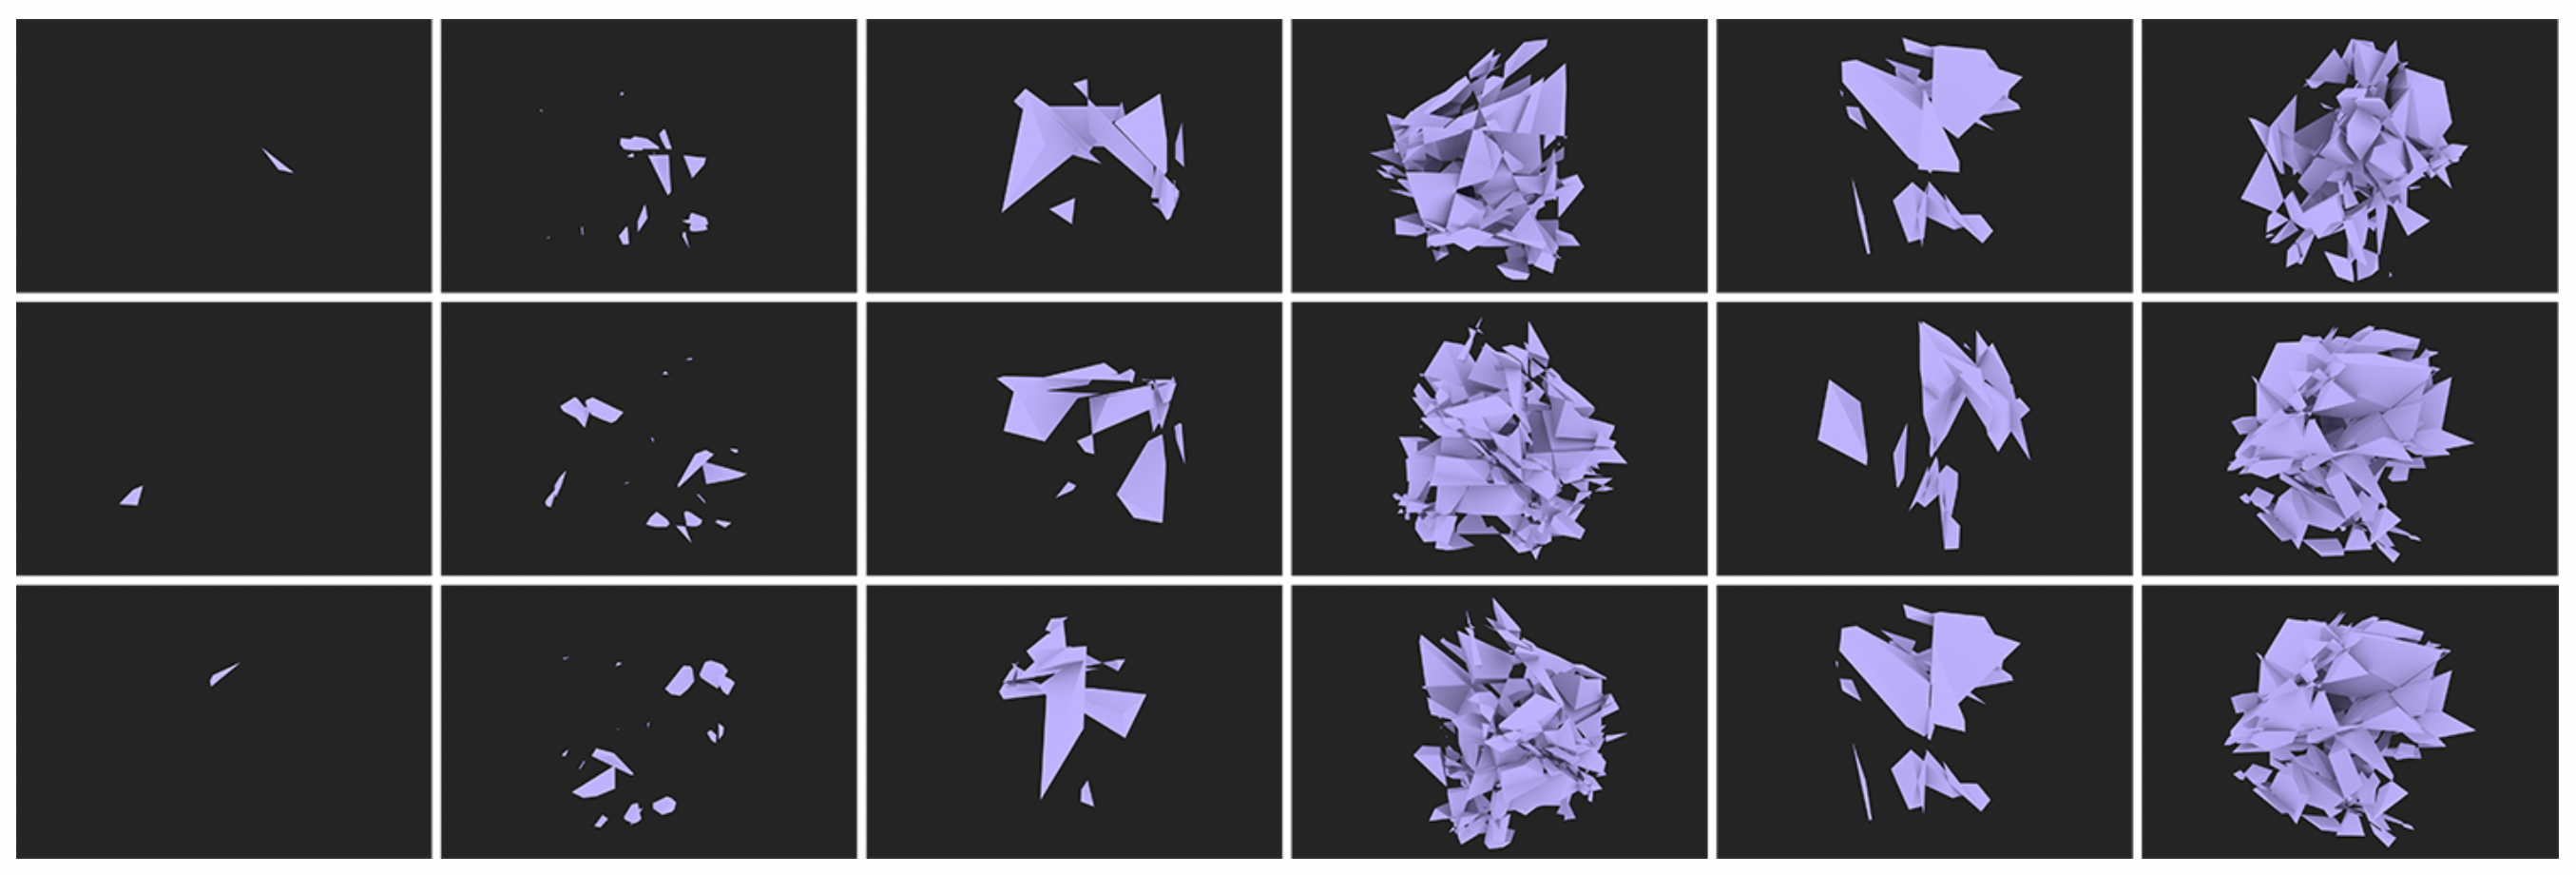
\includegraphics[width=1\columnwidth]{figure/poly1.png}
\caption{Six different scenes (left to right) rendered from three different views (top to bottom). First row: 1 object. Second row: 18 objects and scene layout set to separate. Third row: 18 objects and scene layout set to touching. Fourth row: 180 objects and scene layout set to separate. Fifth row: 18 objects and scene layout set to intersecting. Second row: 100 objects and intersecting layout.}
\label{fig:RPS}
\end{figure*}

\section{Related Work}

This topic, polyhedral recognition, has been studied, both theoretically and empirically, numerous times in different context. As for the theoretical point of view, Kirousis and Papadimitriou proved that having a graph scheme of a polyhedral it is NP-Complete to either decide a legal labeling for them or state whether it is a projection of a given scene\cite{10.1007/3-540-16766-8_17}. Furthermore, Tsotsos presented two theorems regarding the complexity of Visual Search. These theorems show that Unbounded Visual Search is NP-Complete while Bounded Visual Match has linear time complexity. These theorems point out the fact that knowledge of the scene reduces the complexity of this particular problem\cite{tsotsos1989complexity}. These studies have a number of implications. They first tell us that the data-directed approach to vision is computationally intractable in the general case. Meaning that to solve a vision problem solely based on data, one needs to obtain an uncountable number of images which is not feasible. They also tell us that bounded visual search takes time linearly dependent on the size of the input \cite{wolfe2015visual}. Also, even small amounts of task guidance can turn an exponential problem into one with linear time complexity.
\\

\noindent All the aforementioned theoretical proofs are for the case of a single image input; hence one might wonder, considering the fact that scene knowledge reduces the time complexity of recognition task, does having multiple view-points change NP-Completeness also? This simple question is the bridge between active perception and object recognition \cite{ffkf}. Active perception is the case in which an active observer has the ability of acquire multiple-view points from a scene. Such a system naturally has to solve a number of sub-tasks including finding the next best position and/or camera configuration.

\section{Methodology}
\subsection{Problem Settings}

Given two polyhedral scene IDs $\{I_1, I_2\}$ decide whether the underlying 3D objects are the same or not. To solve this challenge one should follow an active vision scheme in which each observations are denoted as $\{ F_i^n, F_j^m \}_{n, m = 1}^{N}$ in which $i$ and $j$ are object indexes and N is the maximum number of view-points taken from an object. that being the case my algorithm consists of four major modules: observation, feature extraction, comparison, and motion policy Fig~\ref{fig:chain}.


\begin{figure*}[t]
\centering
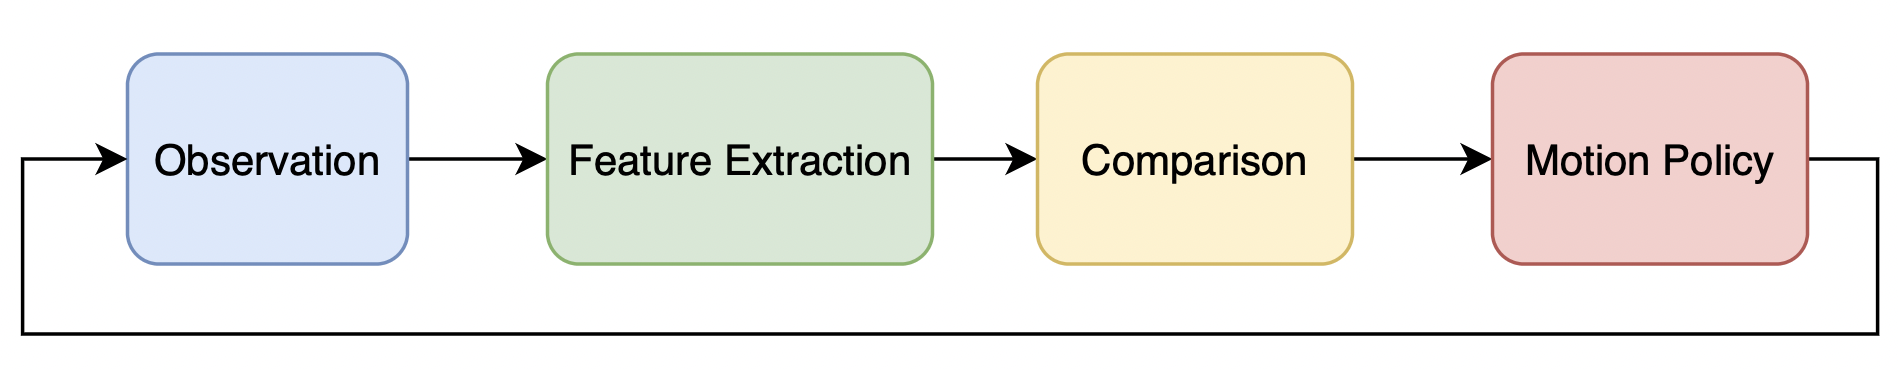
\includegraphics[width=0.9\columnwidth]{figure/module.png}
\caption{Illustration of four main modules of system}
\label{fig:chain}
\end{figure*}

\subsection{Observation \label{subsection:observation}}

\noindent For the observation part I am using the on-demand API. This API provides an easy way of getting rendered images from the polyhedral scenes only by providing a few hyper parameters for camera configuration. These hyper parameters include ID, camera coordinates($x, y, z$), orientating as quaternion($Q_w, Q_x, Q_y, Q_z$), and lightning condition. In my setting I am assuming that the camera is always looking at the origin. With that in mind, the camera location can be represented via a spherial coordinate system ($r, \phi, \theta$). Furthermore, using the pixel intensity of object, I will adjust the $r$ parameter so that a fixed percentage of vertical and/or horizontal internsity is filled with the object. In that case camera position can be denoted with only two parameters $\phi, \theta$. Similar to previous works, I will consider a discrete step size of these two parameter; meaning that they can only obtain values which are a multiplier of $\pi/6$.

\begin{figure*}[t]
\centering{}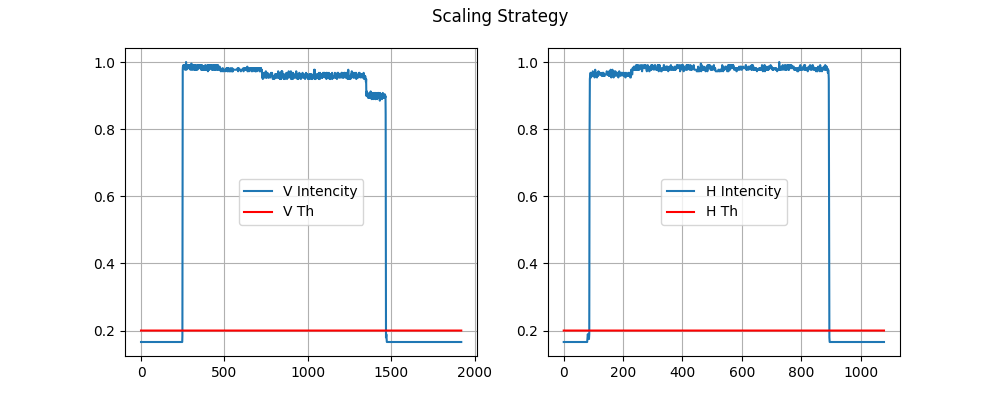
\includegraphics[width=0.95\columnwidth]{figure/scaling.png}
\caption{\label{fig:scaling} Scaling mechanism to determine $r$}
\end{figure*}

\subsection{Feature Extraction \label{subsection:observation}}
\noindent The feature extraction part itself consists of 6 parts: pre-processing, edge detection, line detection, intersecting lines, clustering joints, and graph representation. In this section each part will be explained.
\begin{figure*}[t]
\centering{}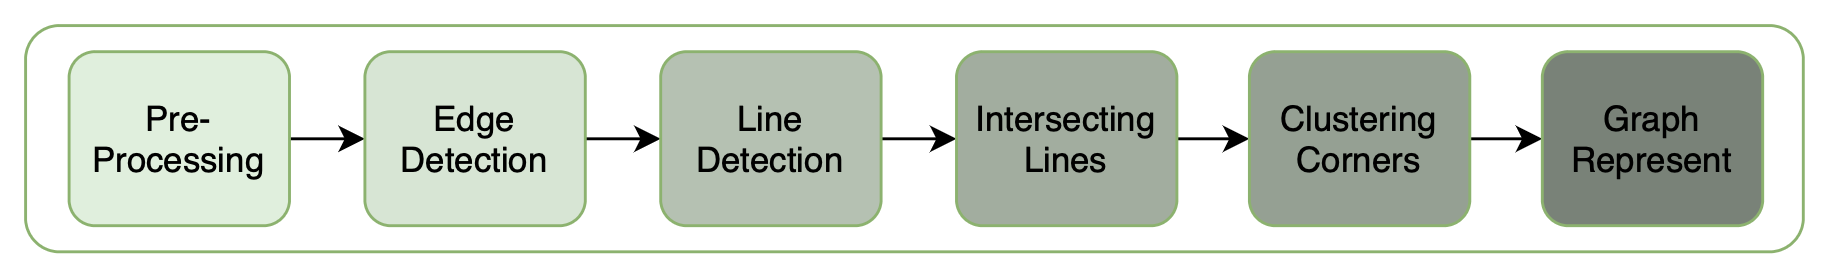
\includegraphics[width=0.95\columnwidth]{figure/features.png}
\caption{\label{fig:features} Feature extraction steps}
\end{figure*}

\noindent \textbf{Pre-Processing.} As a the generated polyhedrals all have the same color, in the pre-processing a gray-scale version is generated. After that, all the functions will be aplied to this image. It is worth mentioning that most edge detection bydefault only work with gray-scale images; in that sense this step is inevitable.
\\

\noindent \textbf{Edge Detection.} Edge detection is an image-processing technique, which is used to identify the boundaries (edges) of objects, or regions within an image. Edges are among the most important features associated with images. We come to know of the underlying structure of an image through its edges. Computer vision processing pipelines therefore extensively use edge detection in applications. Edges are characterized by sudden changes in pixel intensity. To detect edges, we need to go looking for such changes in the neighboring pixels. Sobel Edge Detection is one of the most widely used algorithms for edge detection. The Sobel Operator detects edges that are marked by sudden changes in pixel intensity. This approach states that edges can be detected in areas where the gradient is higher than a particular threshold value. In addition, a sudden change in the derivative will reveal a change in the pixel intensity as well. With this in mind, we can approximate the derivative, using a 3×3 kernel. We use one kernel to detect sudden changes in pixel intensity in the X direction, and another in the Y direction. These are the kernels used for Sobel Edge Detection:
\begin{center}
$K_x =$\begin{bmatrix}
-1 & 0 & +1\\
-2 & 0 & +2\\
-1 & 0 & +1
\end{bmatrix}
\qquad 
$K_y =$\begin{bmatrix}
+1 & +2 & +1\\
0 & 0 & 0\\
-1 & -2 & -1
\end{bmatrix}
\end{center}
When these kernels are convolved with the original image, you get a ‘Sobel edge image’. 
If we use only the Vertical Kernel, the convolution yields a Sobel image, with edges enhanced in the X-direction
Using the Horizontal Kernel yields a Sobel image, with edges enhanced in the Y-direction. Let $G_x$ and $G_y$ represent the intensity gradient in the x and y directions respectively. If $K_x$ and $K_y$ denote the X and Y kernels defined above, then the joint XY detection follows the equations below.

$$
G_x = K_x * I \qquad G_y = K_y * I \qquad G_{xy} \sqrt{G_x^2 G_y^2} \qquad \Theta = arcTan(G_y/G_x)
$$

\noindent \textbf{Line Detection.} For the line detection part the Hough Line Transform is used. It is a transform used to detect straight lines only. To apply the Transform, first an edge detection pre-processing is desirable which was covered in the previous section. As you know, a line in the image space can be expressed with two variables $(m, b) or (r, \theta)$ For Hough Transforms, we will express lines in the Polar system. Hence, a line equation can be written as
$$
y = \left(-\frac{cos(\theta)}{sin(\theta)}\right)x + \left( \frac{x cos(\theta) + y sin(\theta)}{sin(\theta)}\right)
$$
\noindent In general for each point $(x_0,y_0)$, we can define the family of lines that goes through that point as $r_\theta=x_0⋅cos\theta+y_0⋅sin\theta$. Meaning that each pair $(r_\theta,\theta)$ represents each line that passes by $(x_0,y_0)$. If for a given $(x_0,y_0)$ we plot the family of lines that goes through it, we get a sinusoid. We can do the same operation above for all the points in an image. If the curves of two different points intersect in the plane $\theta - r$, that means that both points belong to a same line. t means that in general, a line can be detected by finding the number of intersections between curves.The more curves intersecting means that the line represented by that intersection have more points. In general, we can define a threshold of the minimum number of intersections needed to detect a line. This is what the Hough Line Transform does. It keeps track of the intersection between curves of every point in the image. If the number of intersections is above some threshold, then it declares it as a line with the parameters $(\theta,r_\theta)$ of the intersection point.
\\

\noindent \textbf{Line Intersection.} While the edges of the polydedral are important features, having them alone will not be of use as it will not be representative enough. As such, it is possible to extract the corners of the polyhedral too. To do so I am using a hybrid method wich combines the Harris corner detector with my own line intersection algorithm. As for the latter case, once a line equation is given as $y = mx+b$ one can use it to detect the intersection point of two lines. using the following formula:
$$
y_1 = ax+b,\quad y_2 = cx+d \quad \rightarrow \quad P_0 = \left(\frac{d-c}{a-b}, a\frac{d-c}{a-b}+c\right)
$$
This simple idea is combined with Harris corner detection. Corners are regions in the image with large variation in intensity in all the directions. One early attempt to find these corners was done by Chris Harris & Mike Stephens in their paper A Combined Corner and Edge Detector in 1988, so now it is called the Harris Corner Detector. He took this simple idea to a mathematical form. It basically finds the difference in intensity for a displacement of $(u,v)$ in all directions.
$$
E(u,v) = \sum_{x,y} \underbrace{w(x,y)}_\text{window function} \, [\underbrace{I(x+u,y+v)}_\text{shifted intensity}-\underbrace{I(x,y)}_\text{intensity}]^2
$$

\noindent The window function is either a rectangular window or a Gaussian window which gives weights to pixels underneath. We have to maximize this function $E(u,v)$ for corner detection. That means we have to maximize the second term. Applying Taylor Expansion to the above equation and using some mathematical steps (please refer to any standard text books you like for full derivation), we get the final equation as shown below. Then comes the main part. After this, they created a score, basically an equation, which determines if a window can contain a corner or not.

$$
E(u,v) \approx \begin{bmatrix} u & v \end{bmatrix} M \begin{bmatrix} u \\ v \end{bmatrix} \qquad M = \sum_{x,y} w(x,y) \begin{bmatrix}I_x I_x & I_x I_y \\ I_x I_y & I_y I_y \end{bmatrix}
$$
$$
R = \det(M) - k(\operatorname{trace}(M))^2
$$
\\
\noindent \textbf{Clustering Corners.} Since the corners detected in the previous step are far more than the actual corners, a clustering algorithm will be used to cluster them to unified corners. Once they are clustered, the center of each cluster will be used as the new object corner. For this specific task, I chose DBSCAN as it does not require the number of clusters in its hyper parameters. The DBSCAN algorithm views clusters as areas of high density separated by areas of low density. Due to this rather generic view, clusters found by DBSCAN can be any shape, as opposed to k-means which assumes that clusters are convex shaped. The central component to the DBSCAN is the concept of core samples, which are samples that are in areas of high density. A cluster is therefore a set of core samples, each close to each other (measured by some distance measure) and a set of non-core samples that are close to a core sample. There are two parameters to the algorithm, min-samples and eps, which define formally what we mean when we say dense. Higher min-samples or lower eps indicate higher density necessary to form a cluster.
\\

\noindent \textbf{Graph Representation.} Last but not least, once the corners and edges of the polyhedral are extracted, these information will be treated as a underacted graph with scaled edges. This means that an adjacency matrix M is computed for each graph in which nodes are the polyhedral corners and the edges are its corresponding edges. As for the cost of each eadge, it is computed via the pixed distance of corners devided by the camera scale parameter $r$. It is worth mentioning that the index of each corner(node) in the graph is determined by its pixel distance ranking from the mean corner. Using this scheme the produce graph representation $M$ is invariant to scale and orientation.
$$
M = [M_{ij}] \qquad M_{ij} = PixelDist(corner_i, corner_j)/r \quad  or \; =0
$$
\begin{figure*}[t]
\centering{}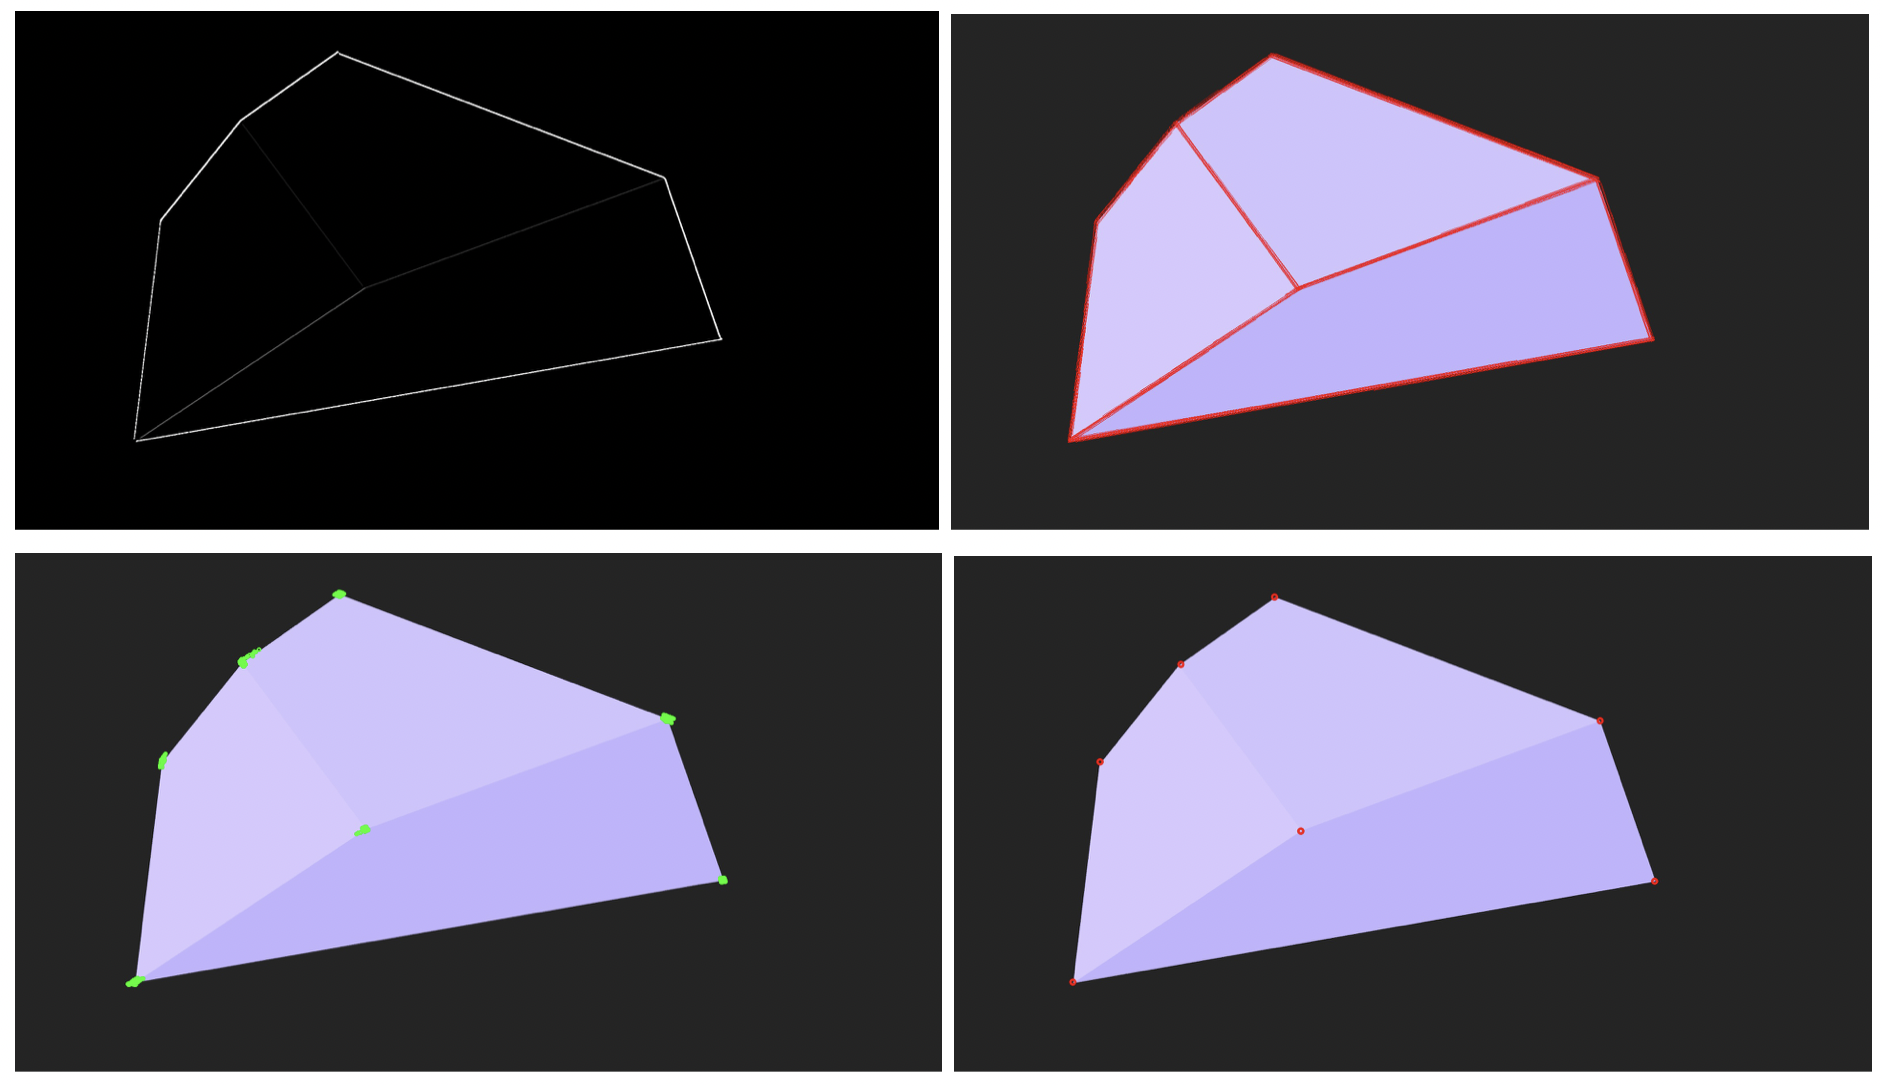
\includegraphics[width=0.95\columnwidth]{figure/ff.png}
\caption{\label{fig:ff}top-left: edges of sobel algorithm, top-right: lines of Hough detection, bottom-left: all the joints detected , bottom-right: center of corner clusters}
\end{figure*}
\\


\subsection{Comparison\label{subsection:network}}
To compare two object the extracted features, adjacency matrices are used in the following way. For a set of image observations $\{ F_i^n, F_j^m \}_{n, m = 1}^{N}$, the corresponding features are denoted as $\{ X_i^n, X_j^m \}_{n, m = 1}^{N}$. Then the distance of two objects is defined as the minimum distance between all feature pairs $\{ X_i^n, X_j^m \}$ as illustrated below.
$$
D(obj_i, obj_j) = min_{m, n}\{d(\{ X_i^n, X_j^m \})\} \qquad d(\{ X_i^n, X_j^m \}) = Mean(abs(M_i^n - M_j^m))
$$

\subsection{Active Motion Policy}
Once the distance of features are computed, there should be a policy deciding what should the next best frame be. Towards that end, with the intuition and corners that are far apart has the potential to present more information, out active policy finds out that specific corner and adjusts the camera location parameters $(\phi, \theta)$ in a way that the chosen corner will be closer to the center of image. Note that these changes in camera coordinates are discrete with step size of $\pi/6$.

\section{Experiment}
For experiments, a nmber of test cases where provided for each students. The answers for the test cases are submitted in a csv file.

\section{Conclusion}
To evaluate the model one should have had grand-truth which was not available for my case. In sum I believe that the approach used in my work follows a common pipeline and hence has room for improvements. A comprehensive evaluation of my solution was not possible as the on demand API has significant latency and therefore capturing a models performance via test cases takes a lot of time. With that said, the proposed solution still has the necessary components of an active vision system and I hope it has reasonable performance.

% \begin{table}[t!]
% \renewcommand\arraystretch{1.2}
% \centering
% \caption{\textbf{Comparisons of tracking results on MOT17 test dataset}.}\label{tab:mot17}
% \scriptsize{
% \setlength{\tabcolsep}{0.55mm}{
% \begin{tabular}{|c|c|cccccccc|c|}

% \hline
% \multicolumn{11}{|c|}{Public Detection} \\
% \hline
% Process & Method & MOTA$\uparrow$ & IDF1$\uparrow$ & MOTP$\uparrow$ & MT$\uparrow$ & ML$\downarrow$ & FP$\downarrow$ & FN$\downarrow$ & IDS$\downarrow$ & Hz$\uparrow$\\
% \hline
% \multirow{4}{*}{Offline} & MHT-bLSTM~\cite{kim2018multi} & 47.5 & 51.9 & {\bf 77.5} & 18.2\% & 41.7\% & 25981 & 268042 & 2069 & {\bf 1.8}\\
% & EDMT~\cite{chen2017enhancing} & 50.0 & 51.3 & 77.3 & {\bf 21.6\%} & 36.3\% & 32279 & {\bf 247297} & 2264 & {\bf 1.8}\\
% & JCC~\cite{keuper2018motion} & 51.2 & {\bf 54.5} & 75.9 & 20.9\% & 37.0\% & 25937 & 247822 & {\bf 1802} & -\\
% & FWT~\cite{Henschel2017} & {\bf 51.3} & 47.6 & 77.0 & 21.4\% & {\bf 35.2\%} & {\bf 24101} & 247921 & 2648 & -\\
% \hline
% \multirow{3}{*}{Online}& DMAN~\cite{zhu2018online} & 48.2 & {\bf 55.7} & 75.9 & 19.3\% & 38.3\% & 26218 & 263608 & 2194 & -\\
% & MOTDT~\cite{chen2018real} & 50.9 & 52.7 & 76.6 & 17.5\% & {\bf 35.7\%} & 24069 & 250768 & 2474 & {\bf 20.6}\\
% & Tracktor~\cite{bergmann2019tracking} & {\bf 53.5} & 52.3 & {\bf 78.0} & {\bf 19.5\%} & 36.6\% & {\bf 12201} & {\bf 248047} & {\bf 2072} & -\\
% \hline
% \hline
% \multicolumn{11}{|c|}{Private Detection} \\
% \hline
% Process & Method & MOTA$\uparrow$ & IDF1$\uparrow$ & MOTP$\uparrow$ & MT$\uparrow$ & ML$\downarrow$ & FP$\downarrow$ & FN$\downarrow$ & IDS$\downarrow$& Hz$\uparrow$\\

% \hline
% \multirow{3}{*}{Online}& Tracktor+CTdet ~\cite{bergmann2019tracking} & 54.4 & 56.1 & 78.1 & 25.7\% & 29.8\% & 44109 & 210774 & 2574&-\\
% & DeepSORT~\cite{wojke2017simple} & 60.3 & {\bf 61.2} & {\bf 79.1} & 31.5\% & {\bf 20.3\%} & 36111 & 185301 & {\bf 2442}&20.0\\
% & {\bf \yang{CTracker} (Ours)} & {\bf 66.6} & 57.4 & 78.2 & {\bf 32.2\%}& 24.2\% & {\bf 22284} & {\bf 160491} & 5529&{\bf 34.4}\\
% \hline
% \end{tabular}}}
% \end{table}

% \iffalse
% \begin{table}
% \renewcommand\arraystretch{1.2}
% \centering
% \caption{Time comparison with SOTA methods on MOT16.}\label{tab:cmp_time}

% \scriptsize{
% \setlength{\tabcolsep}{0.8mm}{
% \begin{tabular}{|c|c|c|c|c|}
% \hline
% Process& Methods&MOTA&Tracking Time (ms)&Tracking FPS\\ \hline
% \multirow{7}{*}{Offline}& MHT-bLSTM~\cite{kim2018multi} & 42.1 & 555.5 & 1.8 \\
% &Quad-CNN~\cite{son2017multi} & 44.1 & 555.5 & 1.8 \\
% &EDMT~\cite{chen2017enhancing} & 45.3& 555.5 & 1.8 \\
% &LMP~\cite{tang2017multiple} &  48.8 & 2000.0 & 0.5 \\
% &NOMT~\cite{choi2015near}&  62.2  & 87.0 & 11.5 \\
% &MCMOT-HDM~\cite{lee2016multi} & 62.4  & {\bf 28.6}  & {\bf 34.9} \\
% &KDNT~\cite{yu2016poi} & 68.2  & 1428.6  & 0.7\\  \hline
% \multirow{5}{*}{Online}&MOTDT~\cite{chen2018real} & 47.6  & 48.5&  20.6  \\
% &EAMTT~\cite{sanchez2016online} & 52.5 & 83.3  & 12.0\\
% &DeepSORT~\cite{wojke2017simple} & 61.4 & 50.0 & 20.0\\
% &CNNMTT~\cite{mahmoudi2019multi} & 65.2  & 89.3  &11.2\\
% &POI~\cite{yu2016poi} & 66.1  & 101.0  & 9.9\\
% &{\bf \yang{CTracker} (Ours)} & {\bf 67.6} & 29.05 & 34.4\\
% \hline
% \end{tabular}}}
% \end{table}
% \fi
\bibliographystyle{splncs}
\bibliography{egbib}
\end{document}
